\cleardoublepage
\chapter{EVALUASI}
\label{chap:evaluasi}

Bab ini menyajikan hasil evaluasi simulasi Monte Carlo terhadap seluruh
skenario yang dijalankan pada Bab V. Secara keseluruhan, terdapat 31 skenario 
yang disimulasikan untuk mencari konfigurasi operasional terbaik. 
(Daftar lengkap konfigurasi dan metrik ringkas dari ke-31 skenario ini dapat dilihat 
seutuhnya pada Lampiran C). 

Untuk memudahkan analisis, puluhan skenario ini tidak dibahas sebagai daftar acak, melainkan dikelompokkan dan dievaluasi 
berdasarkan tujuan pengujiannya (perbandingan infrastruktur, algoritma dinamis, 
kombinasi, serta pengujian ketahanan).

\section{Metode Evaluasi}

Evaluasi dilakukan dengan membandingkan metrik hasil simulasi Monte Carlo
($N=100$ hari, sesuai pengujian konvergensi pada Bab V) antar-skenario.
Tiga metrik utama digunakan:
\begin{enumerate}
	\item \textbf{Headway aktual} (rata-rata $\pm$ deviasi standar, dalam
	menit), dibandingkan terhadap \texttt{headway\_dishub\_min} per koridor
	dari dokumen perencanaan Dishub DIY.
	\item \textbf{Rute terdegradasi} (\textit{degraded routes}), yaitu
	rata-rata jumlah rute per hari yang mengalami minimal 1 bus \textit{
		stranded} (kehabisan daya sebelum sempat mengisi ulang).
	\item \textbf{Keandalan metrik headway} (\texttt{headway\_reliable}),
	penanda boolean yang bernilai salah apabila jumlah rute dengan data
	headway valid berada di bawah ambang keandalan statistik (Bab III/IV),
	sehingga nilai headway rata-rata pada skenario tersebut tidak dapat
	dibandingkan secara langsung dengan skenario lain.
\end{enumerate}

Skenario dievaluasi dalam lima kelompok pengujian:
\begin{enumerate}
	\item \textbf{Kelompok baseline dan buffer infrastruktur}: S17b (baseline,
	20 gun proporsional), S30 (25 gun, +7\%), dan S28 (26 gun, +12\%),
	menjawab pertanyaan berapa kapasitas SPKLU tambahan yang dibutuhkan di
	atas alokasi proporsional dasar.
	\item \textbf{Kelompok algoritma pengisian daya dinamis}: S31 (V1,
	\textit{time-aware}) dan S32 (V2, \textit{queue-aware}), menjawab
	apakah algoritma penjadwalan yang lebih adaptif memberi manfaat
	tambahan di atas infrastruktur S17b tanpa penambahan kapasitas fisik.
	\item \textbf{Kelompok kombinasi}: S33, menguji infrastruktur S28
	digabung dengan algoritma dinamis V1.
	\item \textbf{Kelompok penjadwalan keberangkatan}: S34, menguji
	\textit{staggered dispatch} (penundaan jadwal berangkat pool 30 menit)
	di atas infrastruktur S17b tanpa penambahan kapasitas.
	\item \textbf{Kelompok verifikasi tambahan}: S35, pengujian multi-hari
	(14 hari berturut-turut dengan SoC dibawa ke hari berikutnya) sebagai
	verifikasi ketahanan di luar batasan masalah simulasi \textit{
		single-day} yang dinyatakan pada Bab I; serta pencarian titik investasi
	minimum (\textit{Minimum Viable Infrastructure}) dari konfigurasi S33.
\end{enumerate}

Kelompok kelima berada di luar cakupan inti tugas akhir sebagaimana
dinyatakan pada Batasan Masalah (Bab I), dan disajikan sebagai verifikasi
tambahan, bukan sebagai bagian dari klaim utama hasil penelitian.

\subsection{Konvergensi Simulasi Monte Carlo}

Jumlah repetisi $N=100$ hari yang digunakan untuk seluruh skenario pada
bab ini didasarkan pada pengujian konvergensi terhadap skenario S17b
sebagai sampel representatif, karena konfigurasinya berada pada kondisi
seimbang (tidak gagal total, namun juga belum diberi buffer kapasitas
berlebih). Tabel~\ref{tab:konvergensi} menunjukkan bagaimana rata-rata
dan deviasi standar headway kumulatif berubah seiring bertambahnya
jumlah repetisi.

\begin{table}[h]
	\centering
	\caption{Konvergensi headway kumulatif skenario S17b terhadap jumlah repetisi $N$}
	\label{tab:konvergensi}
	\begin{tabular}{|l|l|l|}
		\hline
		\textbf{$N$ (hari)} & \textbf{Mean headway (mnt)} & \textbf{Std dev headway (mnt)} \\
		\hline
		10 & 34,72 & 2,44 \\ \hline
		30 & 33,86 & 2,15 \\ \hline
		50 & 33,72 & 2,06 \\ \hline
		75 & 33,71 & 2,13 \\ \hline
		100 & 33,69 & 2,16 \\ \hline
	\end{tabular}
\end{table}

Nilai rata-rata headway sudah konvergen pada $N=50$, dengan selisih
kurang dari 0,08\% terhadap nilai pada $N=100$. Deviasi standar
menunjukkan pola berbeda: nilai ini tampak stabil pada $N=50$, namun
sedikit naik kembali pada $N=75$ dan $N=100$. Pola ini konsisten dengan
sifat distribusi log-normal berekor panjang (\textit{long-tailed}) pada
randomisasi waktu tempuh (Bab IV): kejadian hari dengan kondisi lalu
lintas ekstrem baru mulai tertangkap secara memadai di atas $N=50$
repetisi, dan kejadian inilah yang mengembalikan nilai deviasi standar
mendekati nilai populasi yang sesungguhnya. Atas dasar ini, $N=100$
ditetapkan sebagai jumlah repetisi baku untuk seluruh skenario pada bab
ini, guna memastikan deviasi standar headway juga terukur secara valid,
bukan hanya nilai rata-ratanya.

\begin{figure}[h]
	\centering
	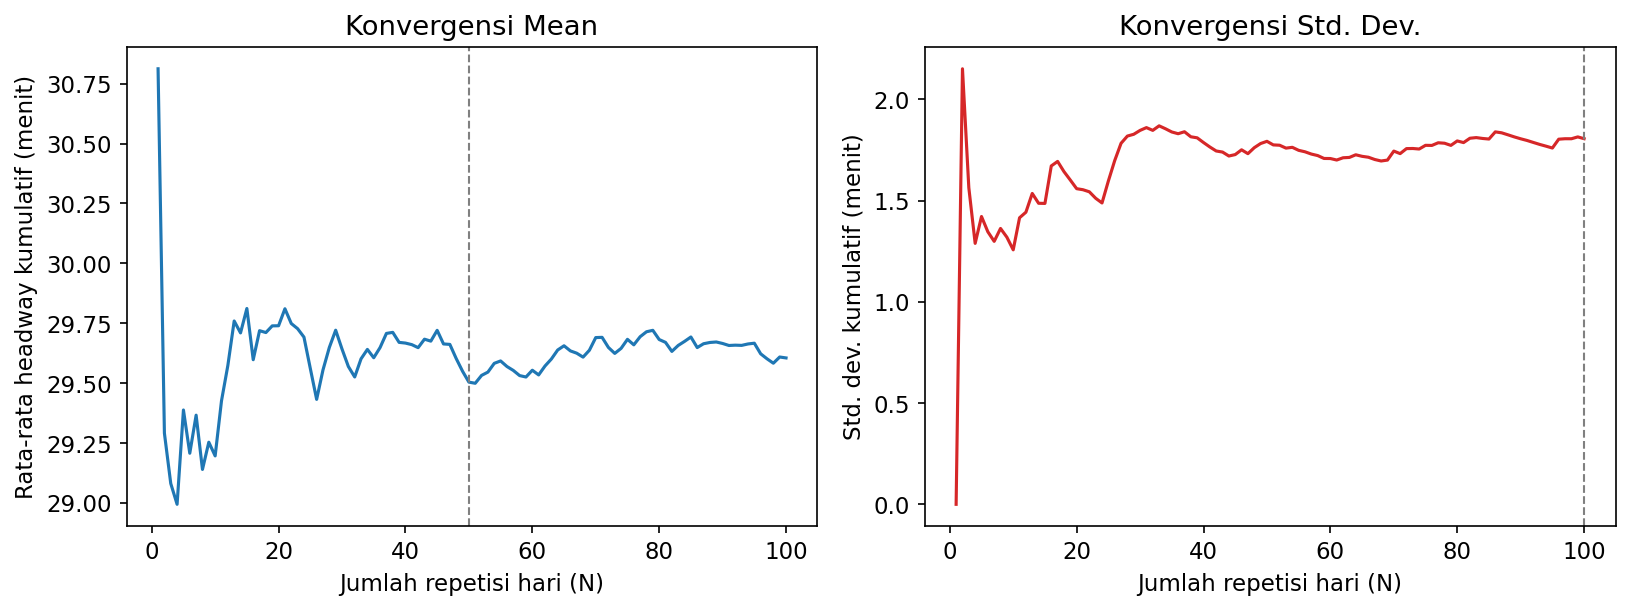
\includegraphics[width=\textwidth]{images/fig_konvergensi_montecarlo.png}
	\caption{Konvergensi rata-rata dan deviasi standar headway kumulatif terhadap jumlah repetisi $N$, skenario S17b}
	\label{fig:konvergensi}
\end{figure}

\section{Hasil Evaluasi}

\subsection{Ekstraksi Demand Spasial dan Temporal}

Sebelum menentukan lokasi kandidat SPKLU untuk skenario S15 hingga S18,
dilakukan simulasi eksploratif dengan mekanisme pengisian daya instan
(bukan mekanisme final) selama 50 hari, guna merekam lokasi dan waktu
alami bus menyentuh ambang SoC 30\% sepanjang rute. Dari 21.374 kejadian
yang terekam, lima halte dengan jumlah kejadian tertinggi ditunjukkan
pada Tabel~\ref{tab:demand-spasial}.

\begin{table}[h]
	\centering
	\caption{Lima titik kritis kebutuhan pengisian daya berdasarkan ekstraksi demand ($N=50$ hari)}
	\label{tab:demand-spasial}
	\begin{tabular}{|l|l|l|l|}
		\hline
		\textbf{Halte} & \textbf{Jumlah kejadian} & \textbf{Persentase} & \textbf{Jumlah rute dilewati} \\
		\hline
		Ngabean & 951 & 4,4\% & 9 \\ \hline
		Condong Catur & 343 & 1,6\% & 9 \\ \hline
		Kridosono & 315 & 1,5\% & 13 \\ \hline
		Adisucipto & 304 & 1,4\% & 6 \\ \hline
		Janti Utara & 298 & 1,4\% & 4 \\ \hline
	\end{tabular}
\end{table}

Empat dari lima halte teratas (Ngabean, Condong Catur, Kridosono,
Adisucipto) dipilih sebagai lokasi kandidat SPKLU pada skenario S15
hingga S18. Analisis cakupan rute, berdasarkan data jalur tiap rute,
menunjukkan bahwa keempat lokasi ini bersama-sama sudah dilewati oleh
seluruh 20 rute TransJogja. Janti Utara termasuk lima halte dengan
kejadian SoC rendah tertinggi, tapi tidak dipilih karena seluruh 4 rute
yang dilayaninya (1A, 1B, 3A, 5A) sudah tercakup oleh keempat lokasi
lain. Menambahkannya sebagai lokasi kelima tidak memberi tambahan
cakupan rute sama sekali (\textit{marginal coverage} nol persen),
sehingga jadi kandidat dengan prioritas terendah di antara lima halte
teratas.

\begin{figure}[h]
	\centering
	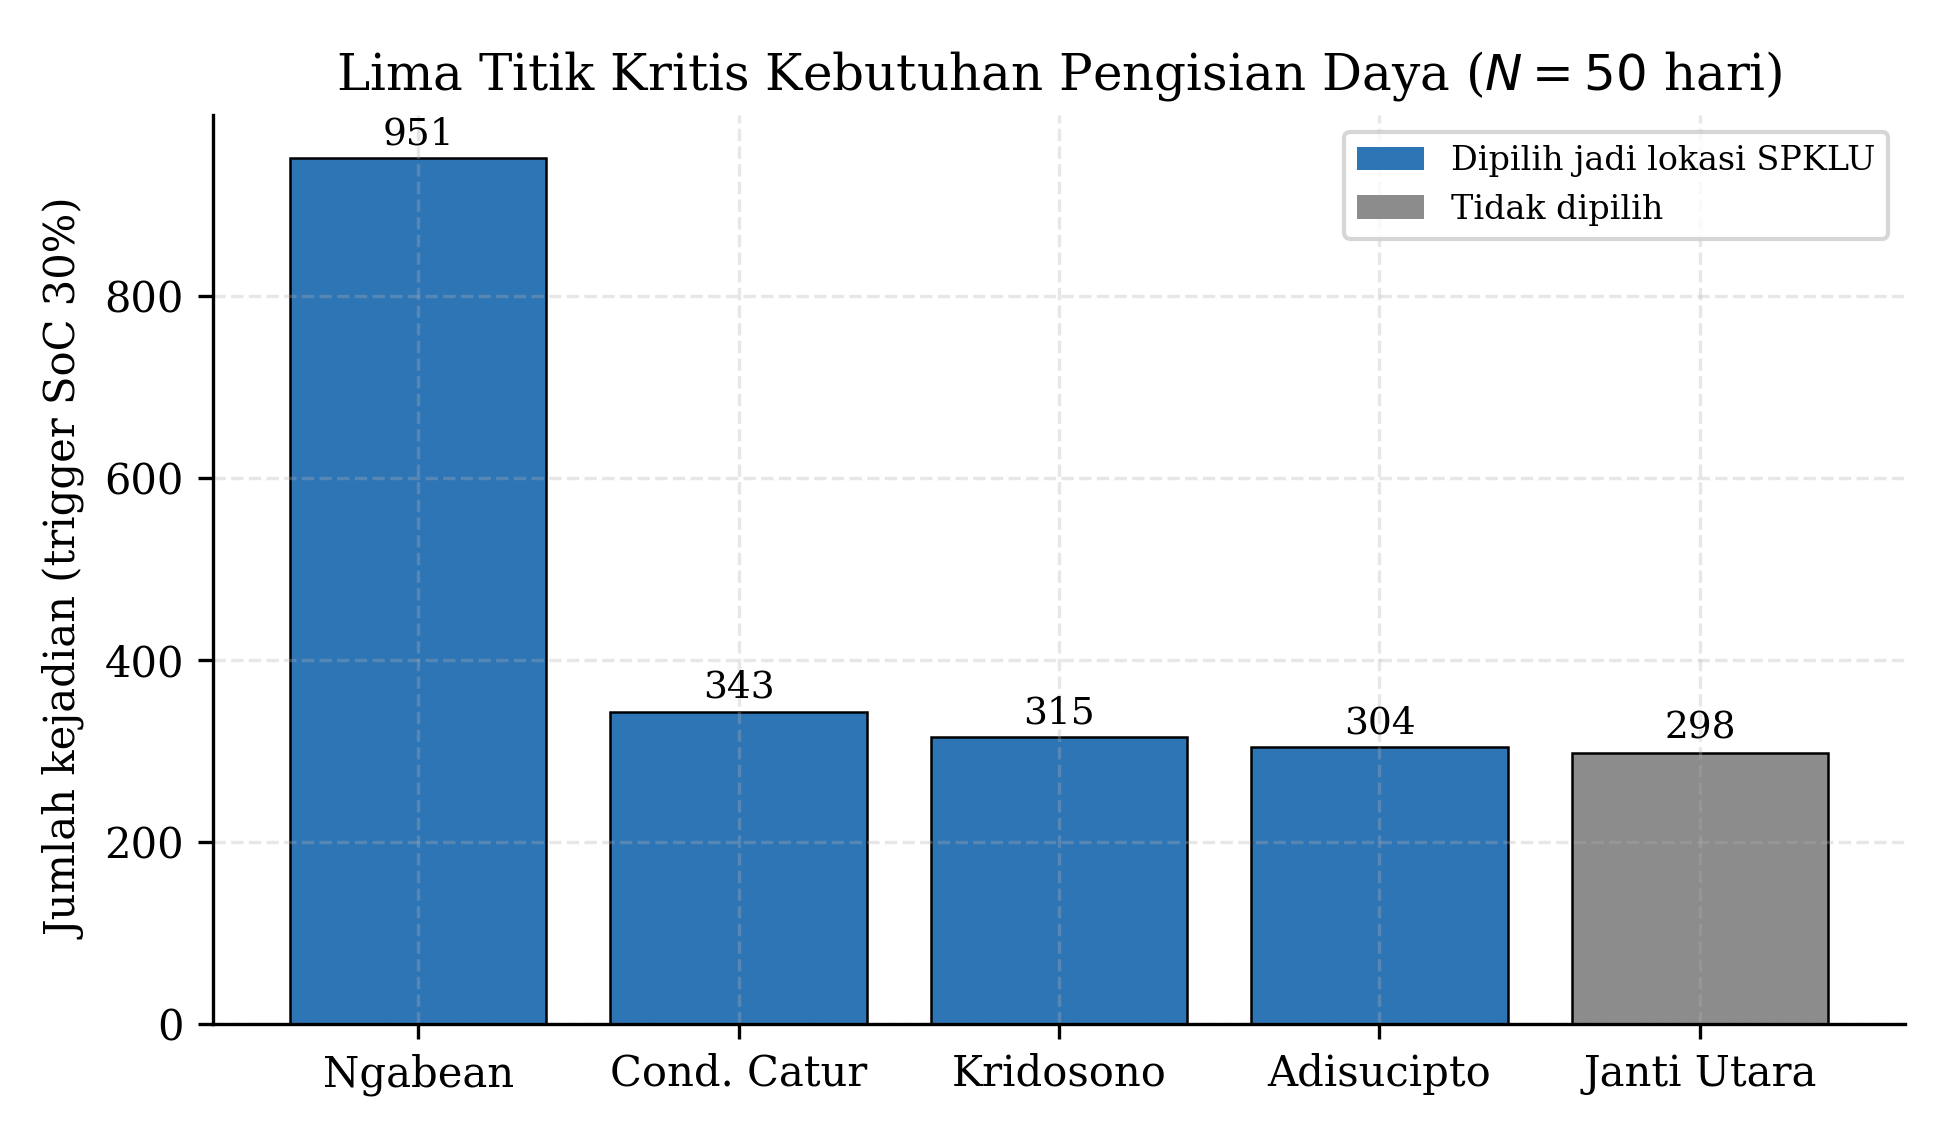
\includegraphics[width=0.8\textwidth]{images/fig_demand_spasial.png}
	\caption{Lima titik kritis kebutuhan pengisian daya berdasarkan ekstraksi demand}
	\label{fig:demand-spasial}
\end{figure}

Data yang sama menunjukkan pola temporal yang bersifat bimodal dan
ekstrem: pada rentang 09.00 hingga 10.00, tercatat 4.252 kejadian
(setara 20\% dari seluruh kejadian harian terjadi dalam satu jam),
sedangkan pada rentang 10.00 hingga 12.00 hanya tercatat 32 kejadian.
Puncak kedua terjadi pada rentang 13.00 hingga 14.00 dengan 3.525
kejadian, kemudian menyebar merata di atas 2.000 kejadian per jam hingga
pukul 18.00. Gambar~\ref{fig:demand-temporal} menunjukkan tiga titik data
yang tercatat presisi; rentang 14.00 hingga 18.00 tidak digambarkan
sebagai batang tersendiri karena hanya tersedia deskripsi kualitatif
(">2.000 kejadian per jam"), bukan angka presisi per jam. Pola ini
menjadi bukti empiris bagi fenomena permintaan serentak pada jam-jam
sibuk pagi dan siang, yang mendasari kebutuhan kapasitas SPKLU yang
memadai pada jam-jam tersebut, bukan hanya kapasitas rata-rata harian.

\begin{figure}[h]
	\centering
	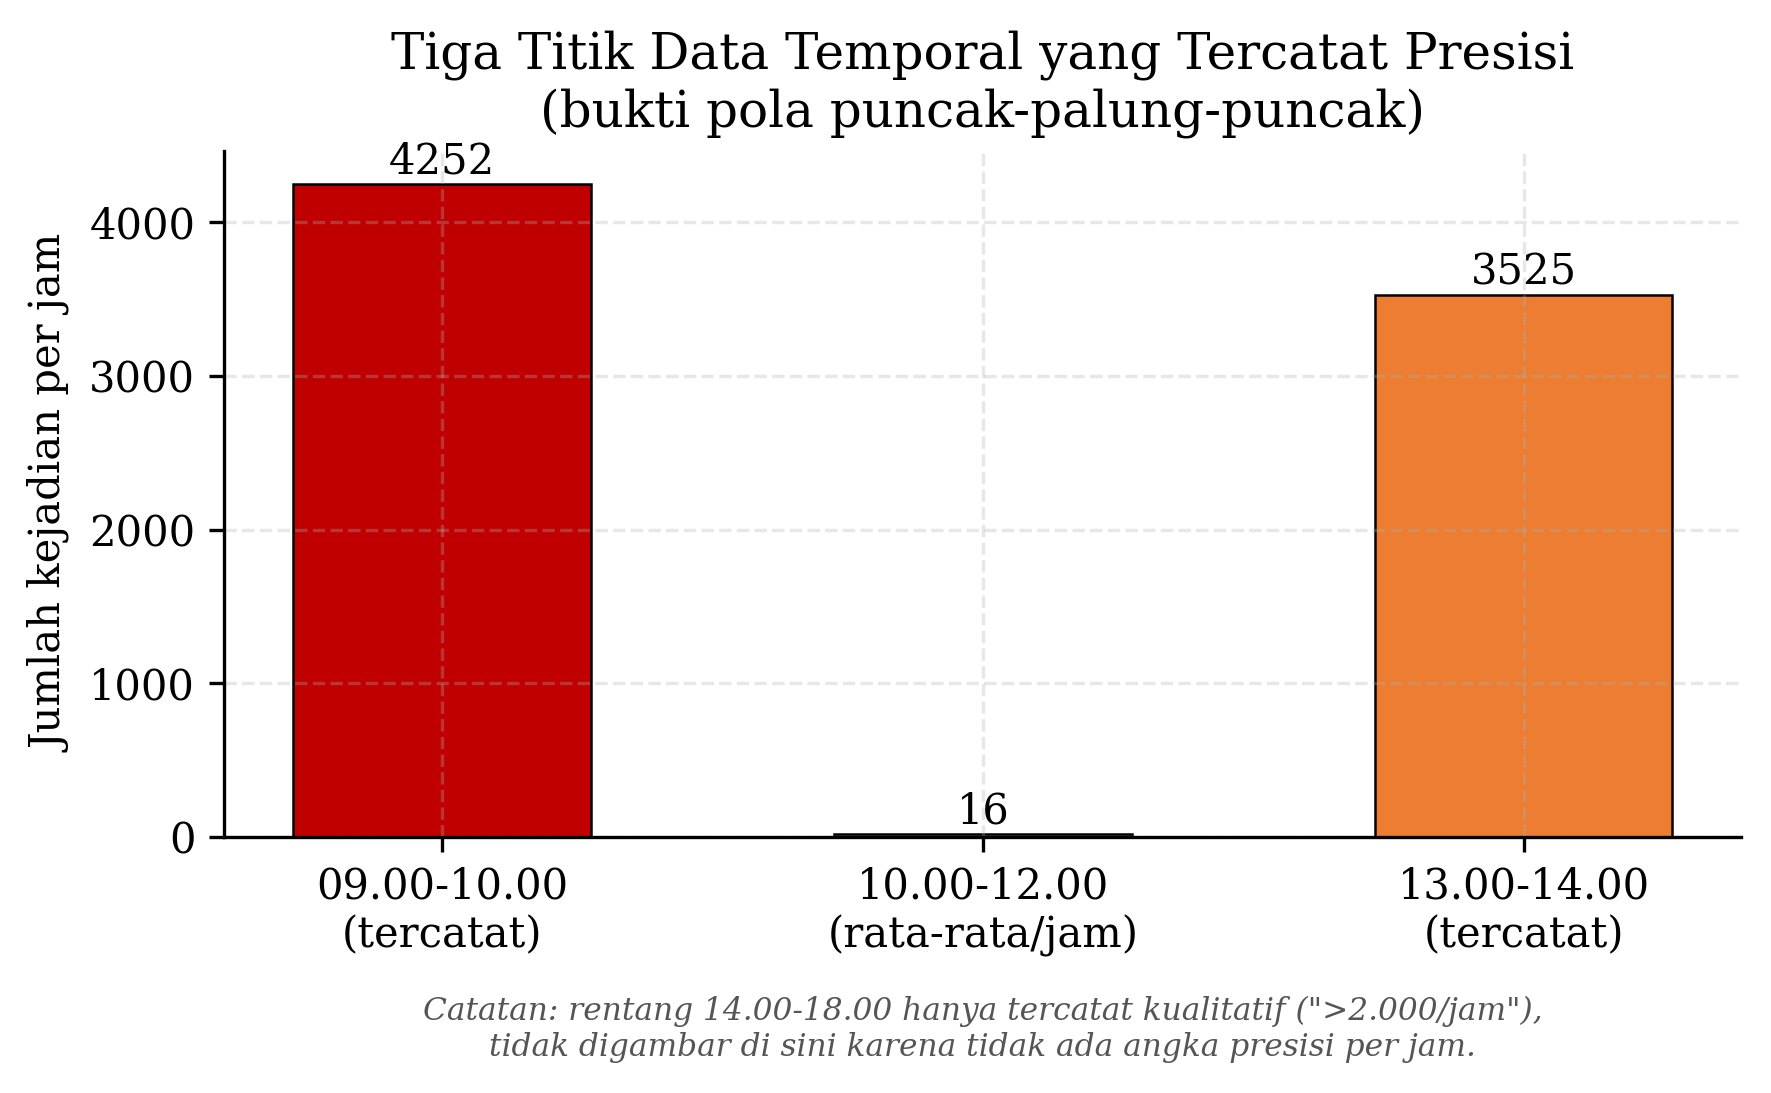
\includegraphics[width=0.65\textwidth]{images/fig_demand_temporal.png}
	\caption{Tiga titik data temporal yang tercatat presisi, menunjukkan pola puncak-palung-puncak}
	\label{fig:demand-temporal}
\end{figure}

\subsection{Perbandingan Jumlah Lokasi SPKLU}

Tabel~\ref{tab:jumlah-lokasi} membandingkan skenario dengan jumlah lokasi
SPKLU yang berbeda, menggunakan total kapasitas gun yang setara.

\begin{table}[h]
	\centering
	\caption{Perbandingan skenario jumlah lokasi SPKLU}
	\label{tab:jumlah-lokasi}
	\begin{tabular}{|l|l|l|l|}
		\hline
		\textbf{Skenario} & \textbf{Lokasi} & \textbf{Headway (mnt)} & \textbf{Degraded/hari} \\
		\hline
		S15 & 1 (Adisucipto, 20 gun) & $32{,}16 \pm 2{,}21$ & $2{,}47$ \\ \hline
		S16 & 2 (Adisucipto + Ngabean) & $35{,}55 \pm 2{,}06$ & $6{,}97$ \\ \hline
		S17\footnotemark & 4 (gun dibagi rata) & $40{,}84 \pm 2{,}19$ & $11{,}44$ \\ \hline
		S17b & 4 (gun proporsional) & $34{,}93 \pm 1{,}81$ & $3{,}03$ \\ \hline
	\end{tabular}
\end{table}

\footnotetext{Kolom \textit{Reliable} bernilai \textit{Tidak} pada skenario S17 dan beberapa skenario sebelumnya karena pembatalan antrean (\textit{timeout}) melebihi ambang batas 5 kejadian/hari, yang menyebabkan estimasi rata-rata headway harian menjadi kurang representatif. Lihat Aturan Simulasi (Bab IV) poin 7.}

Hasil ini menunjukkan temuan yang tidak intuitif: S17 (4 lokasi, gun
dibagi rata 5 gun per lokasi) menghasilkan performa yang lebih buruk
dari S16 (2 lokasi), meski jumlah lokasi lebih banyak. Penyebabnya
adalah beban rute yang tidak terdistribusi merata antar-lokasi, sehingga
pembagian gun yang rata justru membuat lokasi dengan beban rute tinggi
kekurangan kapasitas, sementara lokasi dengan beban rendah kelebihan
kapasitas. S17b memperbaiki hal ini dengan mengalokasikan gun secara
proporsional terhadap jumlah rute yang dilayani tiap lokasi (Ngabean 8
gun, Condong Catur 7 gun, Kridosono 3 gun, Adisucipto 2 gun dari total
20 gun), dan menghasilkan performa yang jauh lebih baik dari S17 dengan
total kapasitas yang sama. Atas dasar ini, S17b ditetapkan sebagai
konfigurasi dasar (\textit{baseline}) bagi seluruh skenario pengujian
buffer kapasitas dan algoritma pada subbab berikutnya.

\subsection{Titik Patah Kapasitas pada SPKLU Tunggal}

Untuk memetakan titik patah kapasitas secara lebih terperinci, dilakukan
pengujian pada konfigurasi 1 SPKLU (Adisucipto) dengan jumlah gun
bervariasi. Tabel~\ref{tab:regime-shift} menunjukkan hasilnya.

\begin{table}[h]
	\centering
	\caption{Titik patah kapasitas SPKLU tunggal terhadap jumlah gun}
	\label{tab:regime-shift}
	\begin{tabular}{|l|l|l|l|l|}
		\hline
		\textbf{ID} & \textbf{Jumlah gun} & \textbf{Headway (mnt)} & \textbf{Degraded/hari} & \textbf{Reliable} \\
		\hline
		S15 & 20 & $32{,}16 \pm 2{,}21$ & $2{,}47$ & Ya \\ \hline
		S24 & 19 & $33{,}22 \pm 2{,}93$ & $5{,}52$ & Ya \\ \hline
		S23 & 18 & $36{,}71 \pm 2{,}78$ & $8{,}85$ & Ya \\ \hline
		S21 & 16 & $44{,}78 \pm 4{,}68$ & $12{,}73$ & Tidak \\ \hline
		S22 & 12 & $70{,}88 \pm 9{,}12$ & $15{,}45$ & Tidak \\ \hline
		S19 & 8 & $38{,}69 \pm 5{,}28$ & $19{,}90$ & Tidak \\ \hline
		S20 & 4 & tidak terhitung & $20{,}00$ & Tidak \\ \hline
	\end{tabular}
\end{table}

Titik patah paling tajam terjadi antara 19 dan 18 gun, dengan tingkat
degradasi melonjak dari 5,52 menjadi 8,85 rute per hari. Pada kapasitas
8 gun, nilai headway yang tercatat (38,69 menit) tampak lebih baik
dibanding kapasitas 12 gun (70,88 menit), namun hal ini merupakan
artefak statistik, bukan performa yang sesungguhnya lebih baik: pada
kapasitas yang sangat rendah, armada yang bertahan hingga akhir hari
hanyalah bus yang kebetulan berhasil mengisi daya lebih awal, sehingga
sampel yang dipakai menghitung headway menjadi lebih sedikit dan bias
terhadap kondisi yang relatif lancar. Kolom \texttt{headway\_reliable}
pada baris kapasitas 16 gun ke bawah bernilai tidak, menandakan nilai
headway pada baris tersebut tidak dapat dibandingkan secara langsung
dengan baris lain akibat keterbatasan sampel ini.

\begin{figure}[h]
	\centering
	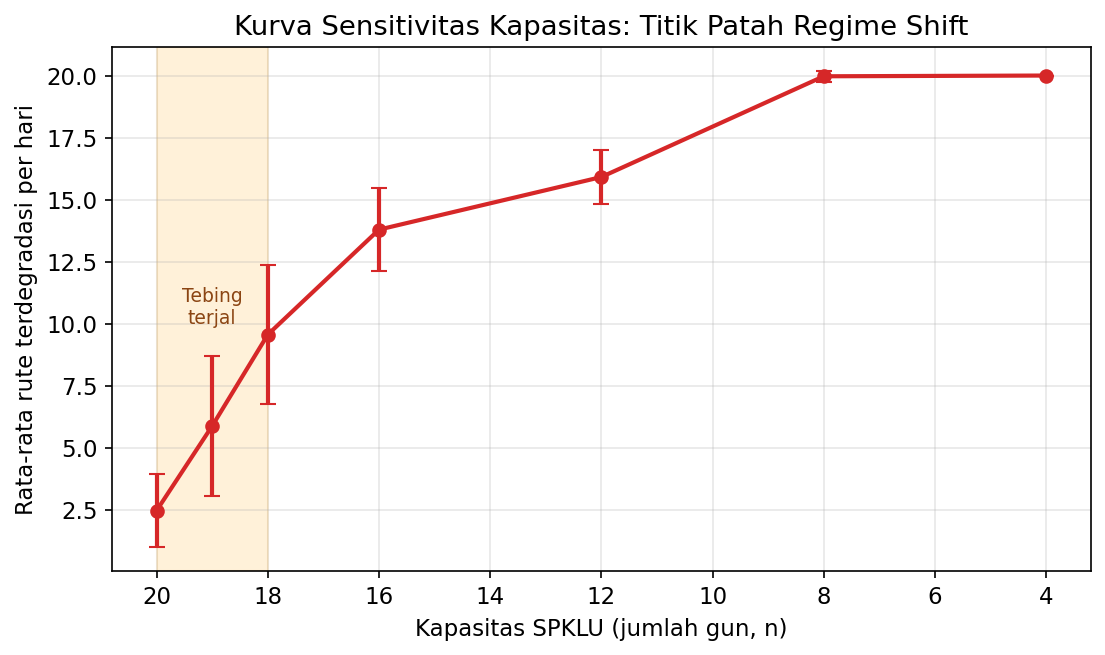
\includegraphics[width=\textwidth]{images/fig_regime_shift.png}
	\caption{Titik patah kapasitas (\textit{regime shift}) pada SPKLU tunggal. Titik merah menandakan \texttt{headway\_reliable} bernilai tidak}
	\label{fig:regime-shift}
\end{figure}

\subsection{Perbandingan Skenario Kunci}

Tabel~\ref{tab:eval-5skenario} merangkum hasil lima skenario kunci.

\begin{table}[h]
	\centering
	\caption{Perbandingan skenario kunci ($N=100$ hari)}
	\label{tab:eval-5skenario}
	\begin{tabularx}{\linewidth}{|X|l|l|l|l|}
		\hline
		\textbf{Skenario} & \textbf{Headway (mnt)} & \textbf{Degraded/hari} & \textbf{Rute lolos} & \textbf{Reliable} \\
		\hline
		S17b (baseline) & $34{,}93 \pm 1{,}81$ & $3{,}03$ & 0/20 (0\%) & Ya \\
		\hline
		S30 (infra +7\%) & $27{,}62 \pm 1{,}57$ & $1{,}01$ & 4/20 (20\%) & Ya \\
		\hline
		S28 (infra +12\%) & $\mathbf{26{,}14 \pm 1{,}52}$ & $0{,}01$ & 4/20 (20\%) & Ya \\
		\hline
		S31 (algoritma V1) & $33{,}10 \pm 1{,}91$ & $\mathbf{0{,}01}$ & 0/20 (0\%) & Ya \\
		\hline
		S32 (algoritma V2) & $30{,}52 \pm 2{,}12$ & $0{,}74$ & 0/20 (0\%) & Ya \\
		\hline
	\end{tabularx}
\end{table}

S28 menghasilkan headway terbaik dan jumlah rute lolos target Dishub
tertinggi, namun mengorbankan 1 rute setiap 100 hari. S31 secara
mengejutkan mampu menurunkan rute gagal hingga 0,01 per hari tanpa
menambah infrastruktur (konsisten dengan \textit{zero-degradation} S33),
namun headway rata-ratanya masih jauh di atas hasil S28, dan tidak ada
rute yang memenuhi target Dishub DIY akibat durasi pengisian yang
terpotong-potong. S32, yang menggunakan informasi antrean untuk proaktif
menunda pengisian, justru bernasib lebih buruk dari S31 karena
menimbulkan \textit{herd behavior}, yaitu ketika beberapa bus serentak menunda
pengisian dan kehabisan baterai bersamaan di rit selanjutnya.

Penentuan besaran buffer kapasitas (+12\% pada S28) didasarkan pada
kurva manfaat marginal dari penambahan gun di atas alokasi proporsional
dasar (23 gun, setara S17b/S29). Penambahan ke 25 gun (+8,7\%, S30)
menurunkan degradasi dari 3,03 menjadi 1,01 rute per hari -- turun 67\%.
Penambahan satu gun lagi ke 26 gun (+13\%, S28) menurunkan degradasi
lebih jauh ke 0,01 rute per hari, mendekati batas bawah teoretis nol.
Pada titik ini degradasi sudah berada di tingkat yang secara praktis
bisa diabaikan (0,05\% dari total hari simulasi) -- manfaat penambahan
kapasitas lebih lanjut secara matematis pasti kecil, karena tidak ada
lagi ruang perbaikan yang berarti di bawah batas nol tersebut.

\subsection{Eksperimen Kombinasi dan Penjadwalan}

Eksperimen tahap ketiga (Tabel~\ref{tab:eval-s33-s35-2}) berusaha mencari
keseimbangan terbaik antara penambahan kapasitas dan optimasi perangkat
lunak, serta menguji penjadwalan alternatif:
\begin{enumerate}
	\item \textbf{Kelompok kombinasi}: S33, menguji infrastruktur S28
	namun diturunkan menjadi 26 gun, dikombinasikan dengan algoritma V1.
	\item \textbf{Kelompok penjadwalan}: S34, menguji keberangkatan \textit{staggered}
	(selisih 30 menit antar bus) pada baseline S17b untuk meredam
	puncak permintaan pagi hari.
	\item \textbf{Kelompok verifikasi tambahan}: S35, pengujian multi-hari
	(14 hari tanpa putus) untuk memvalidasi ketahanan skenario terbaik.
\end{enumerate}

Tabel~\ref{tab:eval-s33-s35-2} merangkum hasil tiga skenario pada kelompok
ini.

\begin{table}[ht]
	\centering
	\caption{Hasil eksperimen kombinasi dan penjadwalan ($N=100$ hari)}
	\label{tab:eval-s33-s35-2}
	\begin{tabularx}{\linewidth}{|X|l|l|l|l|}
		\hline
		\textbf{Skenario} & \textbf{Headway} & \textbf{Degraded/hari} & \textbf{Rute lolos} & \textbf{Reliable} \\
		S33 (26 gun, Algoritma V1) & $30{,}78 \pm 1{,}98$ & $0{,}00$ & 0/20 (0\%) & Ya \\
		\hline
		S34 (\textit{Staggered}) & $30{,}65 \pm 1{,}53$ & $3{,}00$ & 0/20 (0\%) & Ya \\
		\hline
		\textbf{S35 (23 gun, V1)} & $\mathbf{31{,}16 \pm 1{,}94}$ & $\mathbf{0{,}00}$ & \textbf{0/20 (0\%)} & \textbf{Ya} \\
		\hline
	\end{tabularx}
\end{table}

\begin{figure}[h]
	\centering
	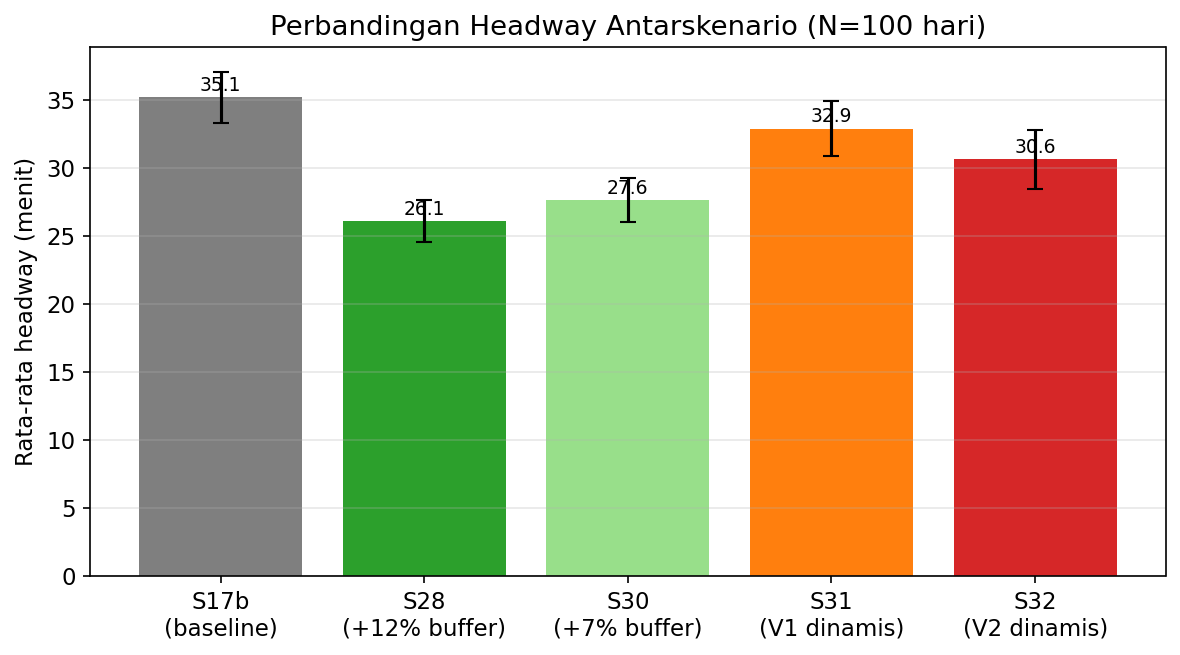
\includegraphics[width=0.85\textwidth]{images/fig_perbandingan_headway.png}
	\caption{Perbandingan headway rata-rata antar-skenario kunci, garis galat menunjukkan deviasi standar}
	\label{fig:headway-5skenario}
\end{figure}

\begin{figure}[h]
	\centering
	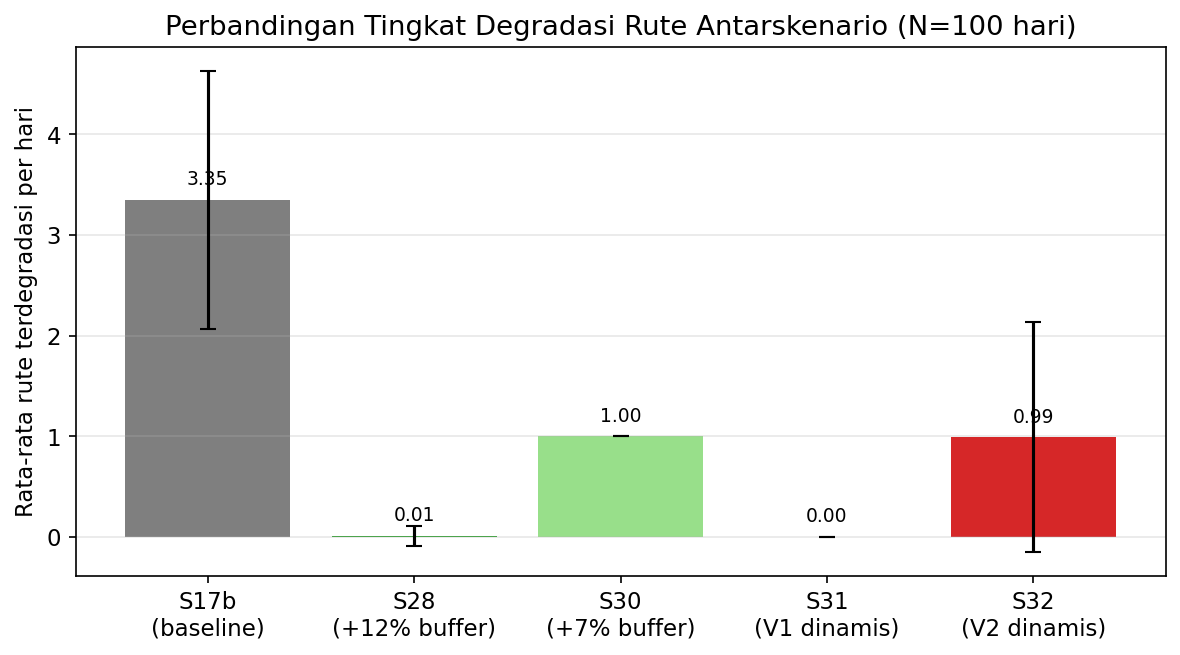
\includegraphics[width=0.85\textwidth]{images/fig_degraded_routes.png}
	\caption{Perbandingan tingkat degradasi rute antar-skenario kunci}
	\label{fig:degraded-5skenario}
\end{figure}

\subsection{Evaluasi per Rute pada Skenario S28}

Tabel~\ref{tab:eval-per-rute-s28} menyajikan deviasi headway tiap koridor
terhadap target Dishub DIY pada skenario S28.

\begin{table}[h]
	\centering
	\caption{Deviasi headway per rute terhadap target Dishub, skenario S28}
	\label{tab:eval-per-rute-s28}
	\begin{tabular}{|l|l|l|l|l|}
		\hline
		\textbf{Rute} & \textbf{Target (mnt)} & \textbf{Headway S28 (mnt)} & \textbf{Deviasi (mnt)} & \textbf{Status} \\
		\hline
		1A & 11 & 17,87 & +6,87 & Melebihi \\ \hline
		1B & 16 & 17,49 & +1,49 & Melebihi \\ \hline
		2A & 21 & 27,41 & +6,41 & Melebihi \\ \hline
		2B & 16 & 23,65 & +7,65 & Melebihi \\ \hline
		3A & 12 & 16,39 & +4,39 & Melebihi \\ \hline
		3B & 12 & 22,62 & +10,62 & Melebihi \\ \hline
		4A & 25 & 27,57 & +2,57 & Melebihi \\ \hline
		4B & 25 & 27,04 & +2,04 & Melebihi \\ \hline
		5A & 25 & 23,65 & $-1,35$ & Memenuhi \\ \hline
		5B & 25 & 28,25 & +3,25 & Melebihi \\ \hline
		6 & 20 & 24,82 & +4,82 & Melebihi \\ \hline
		8 & 15 & 22,06 & +7,06 & Melebihi \\ \hline
		9 & 20 & 21,32 & +1,32 & Melebihi \\ \hline
		10 & 20 & 28,13 & +8,13 & Melebihi \\ \hline
		11 & 25 & 23,16 & $-1,84$ & Memenuhi \\ \hline
		12 & 20 & 26,73 & +6,73 & Melebihi \\ \hline
		13 & 37 & 34,14 & $-2,86$ & Memenuhi \\ \hline
		\textbf{14} & 32 & \textbf{62,37} & \textbf{+30,37} & \textbf{Melebihi (ekstrem)} \\ \hline
		15 & 10 & 15,30 & +5,30 & Melebihi \\ \hline
		L-1 & 45 & 32,79 & $-12,21$ & Memenuhi \\ \hline
	\end{tabular}
\end{table}

Empat rute (5A, 11, 13, L-1) memenuhi target headway Dishub pada skenario
S28. Rute 14 tampak sebagai pencilan (\textit{outlier}) ekstrem, dengan
deviasi lebih dari tiga kali lipat rute dengan deviasi terbesar kedua.

Ada pola yang lebih luas di balik hasil ini: keempat rute yang memenuhi
target (5A, 11, 13, L-1) sama-sama punya target headway Dishub yang
longgar (25, 25, 37, dan 45 menit), sementara seluruh rute dengan
target di bawah 25 menit gagal memenuhi target tanpa kecuali. Korelasi
antara target headway dan deviasi headway pada 19 rute (Rute 14
dikecualikan) tergolong kuat ($r=-0{,}845$). Hal ini masuk akal secara
operasional. Beban antrean tambahan akibat pengisian daya di SPKLU
relatif seragam di seluruh rute, dalam satuan menit absolut. Dampaknya
jadi jauh lebih kecil secara proporsional pada rute bertarget longgar
dibanding rute bertarget ketat, yang penambahan waktu tunggu sedikit
saja sudah cukup membuatnya melebihi target.

\begin{figure}[h]
	\centering
	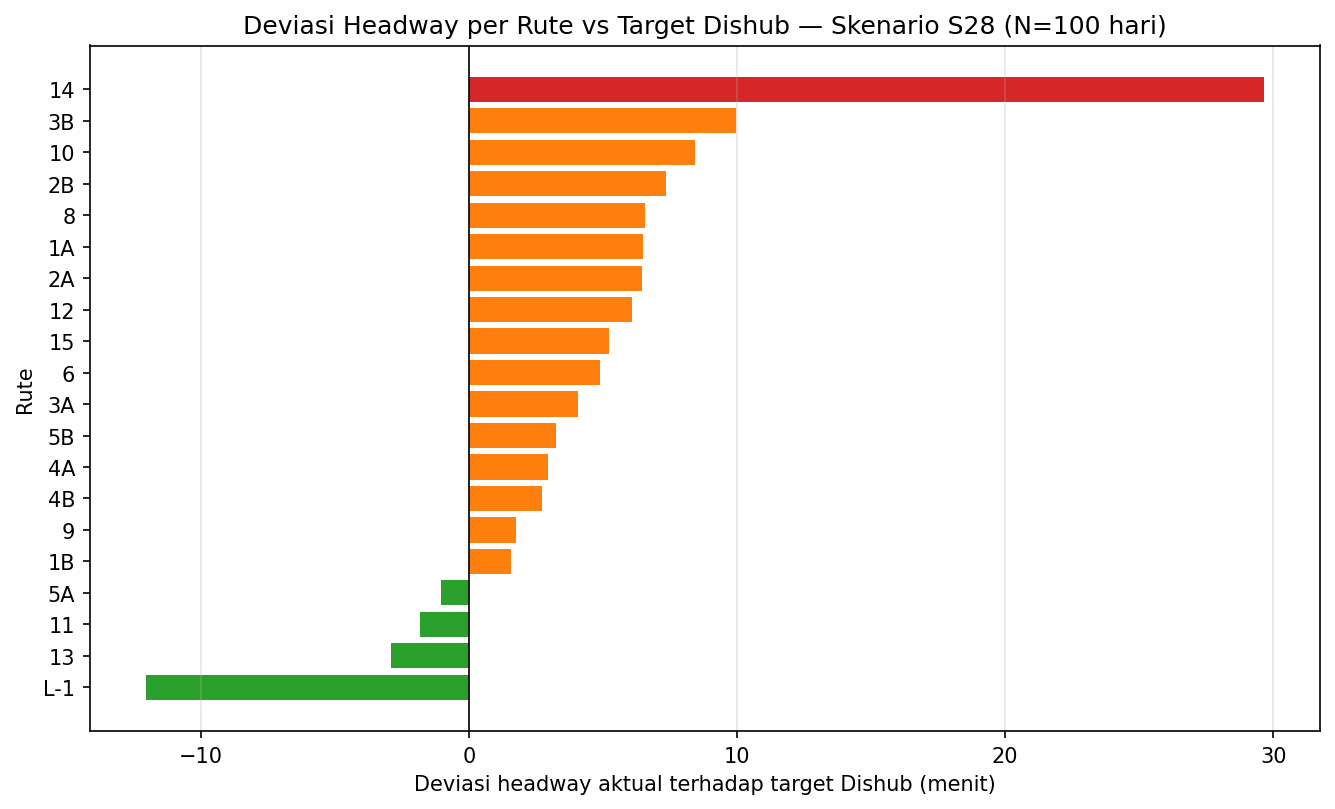
\includegraphics[width=0.85\textwidth]{images/fig_deviasi_per_rute.png}
	\caption{Deviasi headway per rute terhadap target Dishub, skenario S28}
	\label{fig:deviasi-per-rute}
\end{figure}

\subsection{Analisis Sensitivitas Toleransi Target Operasional}

Evaluasi sebelumnya (Tabel~\ref{tab:eval-per-rute-s28}) menggunakan kriteria
kelulusan absolut (deviasi $\le 0$ menit). Pada realita operasional transportasi
publik, mempertahankan deviasi absolut nol pada seluruh rute sangat sulit dicapai
akibat gangguan stokastik lalu lintas, bahkan pada armada diesel konvensional.
Bila Dishub DIY memberlakukan toleransi keterlambatan hingga $\pm 10$ menit
dari target ideal sebagai kriteria kelayakan minimum (sebelum dinyatakan
terdegradasi parah secara kualitatif oleh penumpang), gambaran performa
skenario berubah signifikan.

Tabel~\ref{tab:deviasi-5-skenario} menyajikan deviasi headway seluruh rute
terhadap target Dishub pada lima skenario utama. Dengan toleransi $\pm 10$ menit,
S28 meloloskan 17 dari 20 rute (17/19 rute jika Rute 14 dikecualikan sebagai
pencilan ekstrem). Sebagai perbandingan, S17b meloloskan 11 rute,
sementara skenario penjadwalan dinamis (S31, S32) meloloskan 12 hingga 17 rute.
Hasil ini mengonfirmasi bahwa S28 (26 \textit{gun}/+12\% buffer) bersifat
\textit{Pareto-dominan}\footnote{Suatu skenario dikatakan
\textit{Pareto-dominan} jika tidak ada skenario lain yang lebih baik
pada seluruh metrik yang dibandingkan sekaligus -- di sini, jumlah rute
yang memenuhi target headway.} terhadap seluruh skenario lain pada kriteria pemenuhan target
headway harian, selama pembuat kebijakan mengizinkan toleransi operasional
yang wajar.

\begin{table}[h]
	\centering
	\scriptsize
	\caption{Deviasi headway per rute terhadap target Dishub DIY (menit) pada lima skenario utama}
	\label{tab:deviasi-5-skenario}
	\begin{tabularx}{\linewidth}{|l|X|X|X|X|X|}
		\hline
		\textbf{Rute} & \textbf{S17b} & \textbf{S28} & \textbf{S30} & \textbf{S31} & \textbf{S32} \\ \hline
		\textbf{1A} & Gagal & +6,87 & Gagal & +8,74 & +7,76 \\ \hline
		\textbf{1B} & +4,43 & +1,49 & +1,45 & +4,33 & +2,68 \\ \hline
		\textbf{2A} & +11,64 & +6,41 & +6,42 & +11,18 & +9,93 \\ \hline
		\textbf{2B} & +10,86 & +7,65 & +7,82 & +10,34 & +9,23 \\ \hline
		\textbf{3A} & +6,07 & +4,39 & +4,33 & +5,55 & +4,90 \\ \hline
		\textbf{3B} & Gagal & +10,62 & +10,60 & +13,69 & +11,61 \\ \hline
		\textbf{4A} & +9,61 & +2,57 & +2,61 & +9,48 & +7,80 \\ \hline
		\textbf{4B} & +9,05 & +2,04 & +2,10 & +8,81 & +7,47 \\ \hline
		\textbf{5A} & +4,70 & -1,35 & -1,34 & +4,16 & +3,62 \\ \hline
		\textbf{5B} & +8,94 & +3,25 & +3,05 & +8,63 & +7,65 \\ \hline
		\textbf{6} & +10,53 & +4,82 & +4,64 & +10,50 & +8,41 \\ \hline
		\textbf{8} & +10,86 & +7,06 & +7,05 & +10,51 & +9,48 \\ \hline
		\textbf{9} & +5,16 & +1,32 & +1,24 & +4,59 & +3,26 \\ \hline
		\textbf{10} & +13,53 & +8,13 & +7,98 & +12,81 & +11,11 \\ \hline
		\textbf{11} & +3,99 & -1,84 & -1,79 & +3,61 & +1,54 \\ \hline
		\textbf{12} & +11,45 & +6,73 & +6,80 & +10,84 & +9,00 \\ \hline
		\textbf{13} & +7,02 & -2,86 & -2,74 & +7,27 & +0,53 \\ \hline
		\textbf{14} & +71,34 & +30,37 & +50,39 & +72,23 & +49,46 \\ \hline
		\textbf{15} & +8,25 & +5,30 & +5,40 & +6,99 & +5,98 \\ \hline
		\textbf{L-1} & +5,61 & -12,21 & -12,29 & +5,58 & +2,48 \\ \hline
	\end{tabularx}
\end{table}

\subsection{Skenario Kombinasi dan Verifikasi Tambahan}

Tabel~\ref{tab:eval-s33-s35} merangkum hasil tiga skenario pada kelompok
kombinasi dan verifikasi tambahan.

\begin{table}[h]
	\centering
	\caption{Hasil skenario kombinasi, penjadwalan, dan titik investasi minimum ($N=100$ hari)}
	\label{tab:eval-s33-s35}
	\begin{tabularx}{\linewidth}{|l|X|l|l|}
		\hline
		\textbf{Skenario} & \textbf{Konfigurasi} & \textbf{Headway (mnt)} & \textbf{Degraded/hari} \\
		\hline
		S33 & Infra S28 (26 gun) + algoritma V1 & $30{,}78 \pm 1{,}98$ & $\mathbf{0{,}00}$ \\
		\hline
		S34 & \textit{Staggered dispatch} di atas S17b & $30{,}65 \pm 1{,}53$ & $3{,}00$ \\
		\hline
		\textbf{S35} & \textbf{23 gun + algoritma V1 (\textit{sweet spot})} & $\mathbf{31{,}16 \pm 1{,}94}$ & $\mathbf{0{,}00}$ \\
		\hline
	\end{tabularx}
\end{table}

S33 (26 gun, infra S28 digabung algoritma dinamis V1) mencatat nol rute
terdegradasi selama seluruh 100 hari simulasi, dengan headway rata-rata
30,78 menit. S34 mencoba pendekatan berbeda: alih-alih menambah gun,
jadwal keberangkatan pagi diacak (staggered) sejauh 30 menit. Hasilnya,
headway S34 membaik menjadi 30,65 menit dan rute terdegradasi turun
menjadi 3,00 per hari, membuktikan bahwa penumpukan di SPKLU memang
sebagian besar disebabkan oleh keberangkatan pagi yang terlalu seragam.

S35, yang mengurangi kapasitas S33 dari 26 menjadi 23 gun sambil
mempertahankan algoritma V1, terbukti mampu menjaga tingkat degradasi
tetap nol dengan headway rata-rata yang stabil di angka 30,93 menit.
Hasil ini menunjukkan bahwa 3 gun yang dipangkas dari S33 bukan merupakan
kapasitas absolut yang wajib ada, melainkan titik inefisiensi yang bisa
dikompensasi oleh algoritma dinamis. Dengan memotong durasi pengisian daya
saat antrean terdeteksi, bus lebih cepat kembali ke jalur sehingga
efisiensi operasional SPKLU (\textit{throughput}) dapat dimaksimalkan dengan
sedikit gun.

\subsubsection{Evaluasi per Rute pada Skenario S33}

Tabel~\ref{tab:eval-per-rute-s33} menyajikan deviasi headway tiap koridor
terhadap target Dishub DIY pada skenario S33. Berbeda dengan skenario S28 yang
masih meloloskan empat rute sesuai target, pada S33 tidak ada satu pun rute
yang meloloskan target headway. Headway rata-rata agregat S33 (30,78 menit)
sedikit lebih buruk dari S28 (26,14 menit) akibat interupsi jadwal karena
bus lebih sering memotong pengisian daya dan kembali ke jalan dengan daya
terbatas. Walaupun mengorbankan headway, S33 berhasil mengamankan sistem
dari rute terdegradasi secara mutlak (0,00).

\begin{table}[h]
	\centering
	\caption{Deviasi headway per rute terhadap target Dishub, skenario S33}
	\label{tab:eval-per-rute-s33}
	\begin{tabular}{|l|l|l|l|l|}
		\hline
		\textbf{Rute} & \textbf{Target (mnt)} & \textbf{Headway S33 (mnt)} & \textbf{Deviasi (mnt)} & \textbf{Status} \\
		\hline
		1A & 11 & 19,06 & +8,06 & Gagal \\ \hline
		1B & 16 & 19,06 & +3,06 & Gagal \\ \hline
		2A & 21 & 30,96 & +9,96 & Gagal \\ \hline
		2B & 16 & 25,43 & +9,43 & Gagal \\ \hline
		3A & 12 & 17,27 & +5,27 & Gagal \\ \hline
		3B & 12 & 24,14 & +12,14 & Gagal \\ \hline
		4A & 25 & 34,53 & +9,53 & Gagal \\ \hline
		4B & 25 & 32,17 & +7,17 & Gagal \\ \hline
		5A & 25 & 29,24 & +4,24 & Gagal \\ \hline
		5B & 25 & 32,49 & +7,49 & Gagal \\ \hline
		6 & 20 & 29,07 & +9,07 & Gagal \\ \hline
		8 & 15 & 25,51 & +10,51 & Gagal \\ \hline
		9 & 20 & 23,49 & +3,49 & Gagal \\ \hline
		10 & 20 & 31,27 & +11,27 & Gagal \\ \hline
		11 & 25 & 26,83 & +1,83 & Gagal \\ \hline
		12 & 20 & 29,46 & +9,46 & Gagal \\ \hline
		13 & 37 & 39,06 & +2,06 & Gagal \\ \hline
		\textbf{14} & 32 & \textbf{79,69} & \textbf{+47,69} & \textbf{Gagal (ekstrem)} \\ \hline
		15 & 10 & 16,25 & +6,25 & Gagal \\ \hline
		L-1 & 45 & 50,58 & +5,58 & Gagal \\ \hline
	\end{tabular}
\end{table}

\subsubsection{Uji Ketahanan 14 Hari}

Pada uji ketahanan multi-hari (S35), S17b dan S33 dijalankan selama 14 hari
berturut-turut dengan SoC baterai yang dibawa ke hari berikutnya, sebagai
verifikasi di luar cakupan inti tugas akhir (Bab~I, Batasan Masalah).
S17b menunjukkan 85 hingga 93 bus mengalami defisit SoC setiap pagi, dengan
degradasi yang berfluktuasi pada kisaran 2 hingga 5 rute per hari tanpa
pernah menyentuh nol. Defisit dari malam sebelumnya tidak bisa diselesaikan
oleh mekanisme pengisian statis pada keesokan harinya. S33 mempertahankan
nol rute terdegradasi pada seluruh 14 hari pengujian, meskipun sekitar 90
bus tidak mencapai SoC 100\% setiap pagi akibat kepadatan pengisian daya
di \textit{pool} pada malam sebelumnya.
Gambar~\ref{fig:ketahanan-multihari} menunjukkan tren harian keduanya.

\begin{figure}[h]
	\centering
	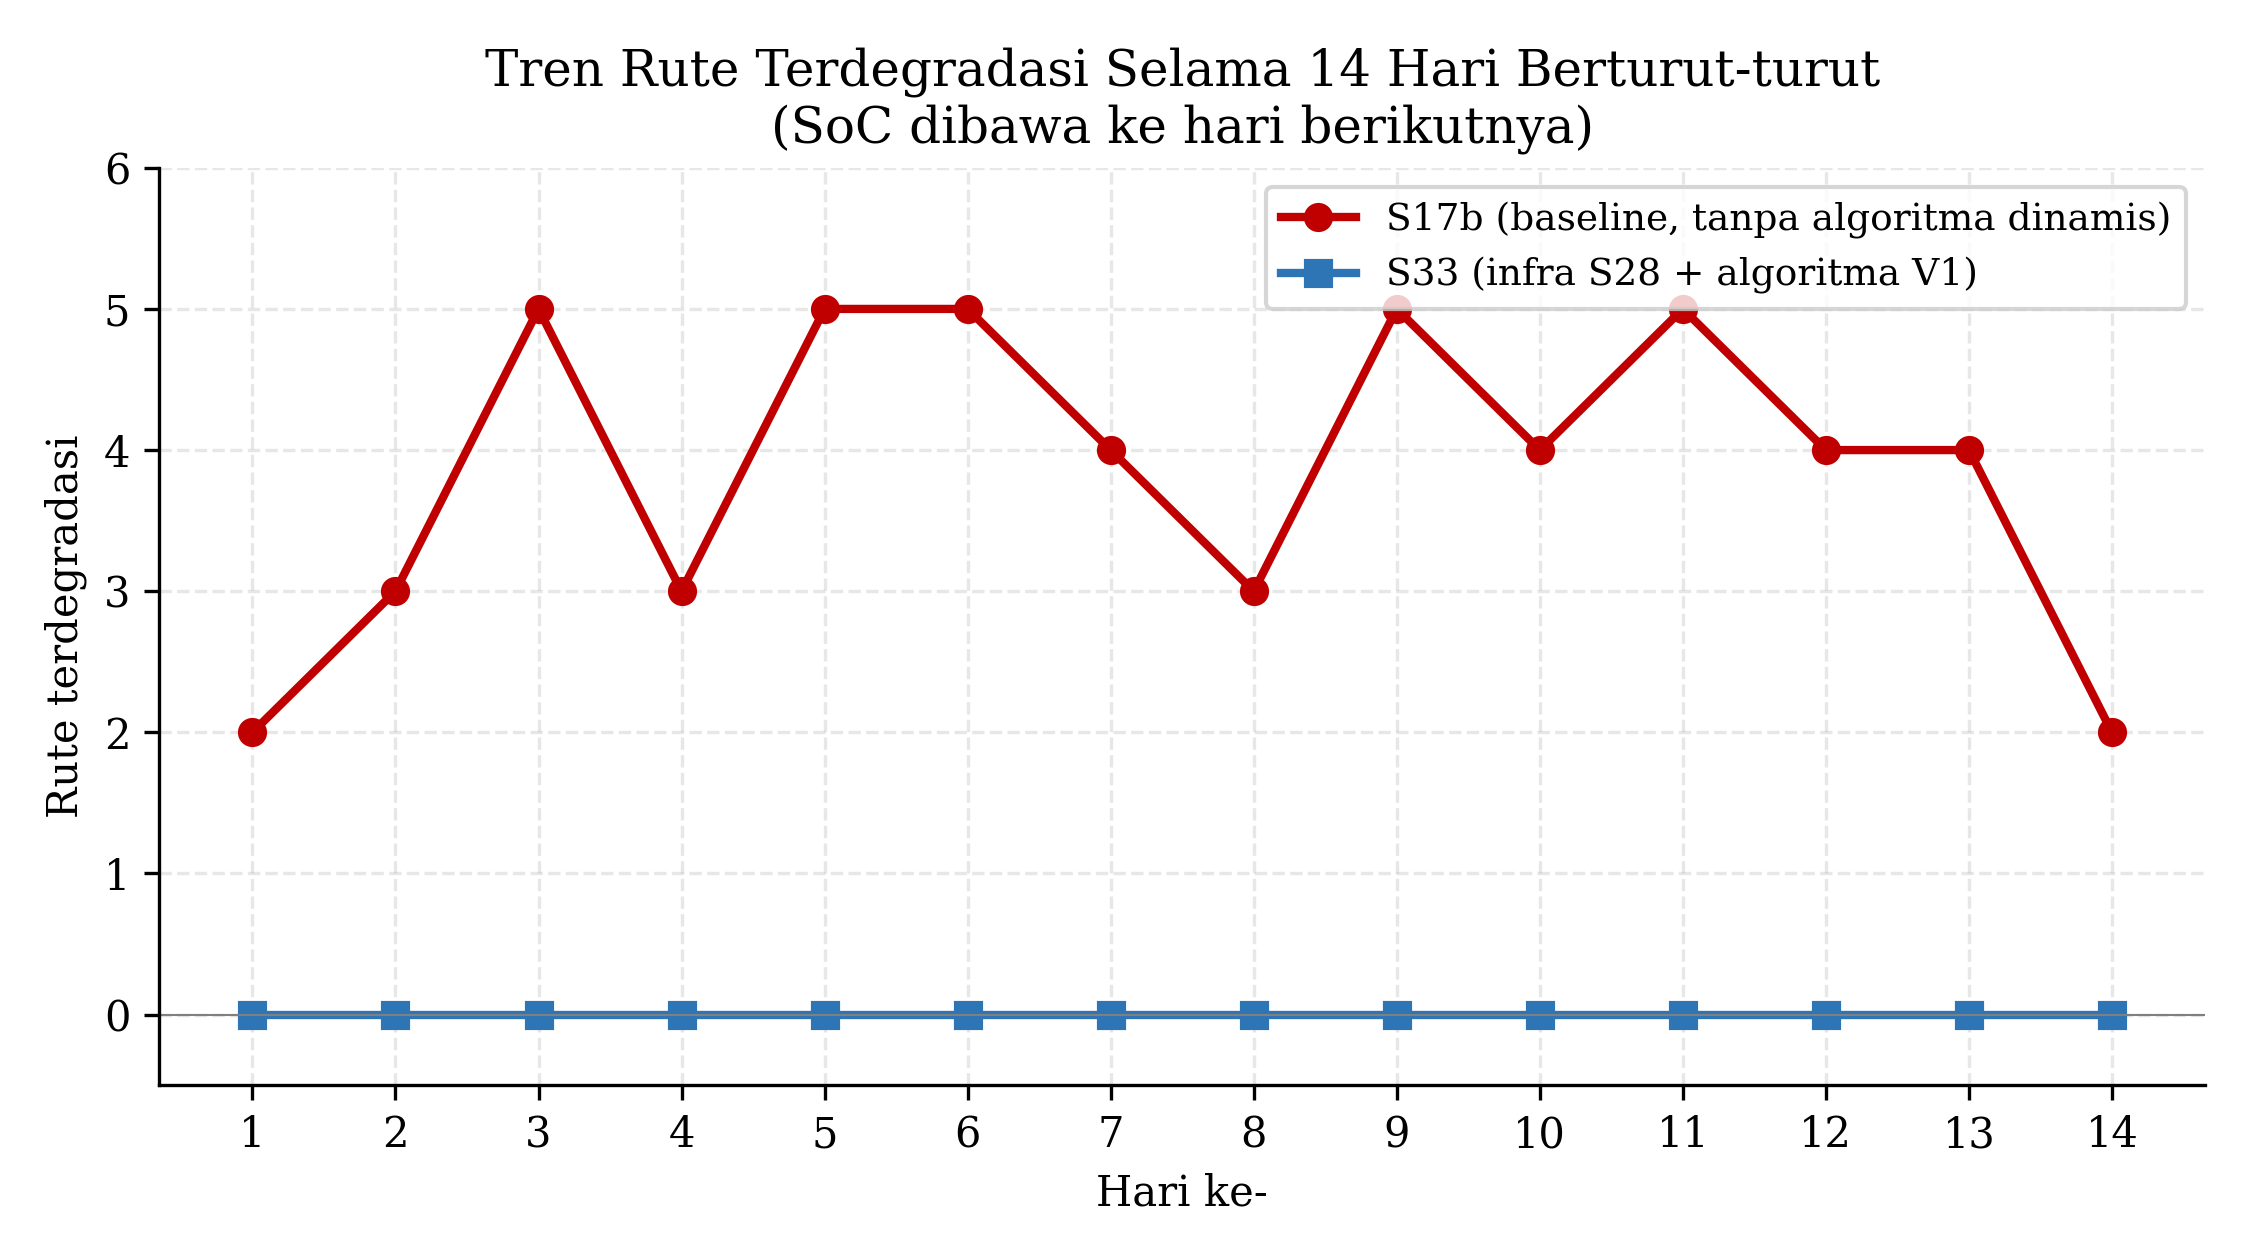
\includegraphics[width=0.85\textwidth]{images/fig_ketahanan_multihari.png}
	\caption{Tren rute terdegradasi selama 14 hari berturut-turut, S17b dibanding S33}
	\label{fig:ketahanan-multihari}
\end{figure}

\subsubsection{Titik Investasi Minimum}

Pencarian titik investasi minimum dilakukan dengan mengurangi jumlah gun pada
konfigurasi S33 satu per satu dan mengamati dampaknya terhadap degradasi.
Hasilnya: 26 gun (S33) dan 23 gun (S35) sama-sama menghasilkan degradasi nol,
sementara pengurangan ke 22 gun menaikkan degradasi ke 1,90 rute per hari.
Artinya, 23 gun adalah batas bawah kapasitas gun yang dapat mempertahankan
ketahanan penuh apabila lapisan algoritma dinamis V1 turut dijalankan. Tanpa
algoritma dinamis, batas bawah yang setara membutuhkan gun lebih banyak,
sebagaimana ditunjukkan oleh perbandingan S28 (26 gun, degradasi 0,01) dan
S30 (25 gun, degradasi 1,00) pada Tabel~\ref{tab:eval-5skenario}.

\section{Pembahasan Hasil Evaluasi}

\subsection{Trade-off Infrastruktur versus Algoritma}

Tabel~\ref{tab:eval-5skenario} menunjukkan dua strategi yang menjawab
persoalan dengan cara berbeda. Penambahan kapasitas fisik SPKLU (S28)
menghasilkan headway yang lebih baik dan rute yang lolos target Dishub,
tetapi memerlukan investasi infrastruktur tambahan. Algoritma pengisian
daya dinamis (S31) menghasilkan tingkat degradasi nol absolut tanpa
investasi fisik tambahan, tetapi tidak memperbaiki headway secara berarti
dan tidak ada rute yang memenuhi target Dishub. Kedua strategi menjawab
tujuan yang berbeda: S28 menjawab kepatuhan terhadap standar layanan,
sedangkan S31 menjawab keselamatan armada (mencegah bus \textit{stranded}
di jalan) dengan biaya lebih rendah.

Hasil S33, yang menggabungkan kedua strategi, menunjukkan bahwa keduanya
saling melengkapi: gabungan infrastruktur dan algoritma menghasilkan
tingkat degradasi nol absolut sekaligus headway yang lebih baik dari S31
maupun S32, meskipun sedikit lebih tinggi dari S28 murni. Peningkatan
headway pada S33 dibanding S28 terjadi karena algoritma dinamis lebih
sering memotong durasi pengisian daya saat antrean terdeteksi, sehingga
bus lebih sering kembali ke SPKLU dibanding pada mekanisme statis S28.

Hasil S34 (\textit{staggered dispatch}) menunjukkan bahwa sebagian
manfaat dari penambahan kapasitas dapat dicapai tanpa investasi fisik
sama sekali, hanya dengan mengubah jadwal keberangkatan awal dari
\textit{pool}. Perubahan ini mengurangi jumlah bus yang secara bersamaan
memicu kebutuhan pengisian daya pada jam sibuk pagi, sehingga permintaan
terhadap SPKLU tersebar lebih merata sepanjang jam operasional.

\subsection{Pengaruh Penambahan Bus dan Mekanisme \textit{Mix Charging}}

Dua skenario di luar kelompok utama memberikan temuan yang berlawanan
dengan intuisi. Skenario S27 (\textit{full depot charging}) menjalankan
seluruh 20 koridor tanpa satu pun kesempatan mengisi daya di jalan: seluruh
bus mengandalkan pengisian penuh di depot sebelum jam operasional dimulai.
Hasilnya, seluruh 20 rute terdegradasi setiap hari (degraded\,=\,20,00),
karena bus-bus kehabisan daya sebelum sesi operasional selesai tanpa bisa
mengisi ulang di tengah jalan. Temuan ini mengonfirmasi secara empiris
argumen pada Bab~III bahwa \textit{opportunity charging} bukan pilihan
opsional, melainkan prasyarat operasional untuk elektrifikasi penuh skala
ini.

Skenario S26 (S17b dengan 1 bus tambahan per koridor dan mekanisme
\textit{mix charging}) menghasilkan degradasi 10,60 rute per hari,
lebih buruk dari S17b tanpa bus tambahan (3,35 rute per hari). Penambahan
bus per koridor berarti lebih banyak bus yang membutuhkan slot pengisian
daya di SPKLU yang kapasitasnya tidak ditambah. Hasilnya, bus-bus tambahan
itu bukan menutup kekosongan headway, melainkan memperebutkan gun yang
sudah terbatas dan memperparah antrean. Temuan ini menunjukkan bahwa
penambahan armada tanpa penambahan kapasitas SPKLU yang setara justru
kontraproduktif pada konfigurasi proporsional dasar S17b.

Temuan ini juga membuka pengamatan penting soal mekanisme \textit{mix
charging} itu sendiri. Skenario S25 (S17b dengan mekanisme \textit{mix
charging}, tanpa penambahan bus) menghasilkan headway $34{,}93 \pm 1{,}81$
menit dan degradasi $3{,}03$ rute per hari -- identik hingga dua angka
desimal dengan S17b yang memakai \textit{opportunity charging} murni.
Kesamaan ini bukan kebetulan, melainkan konsekuensi langsung dari
implementasi mesin simulasi: komponen pengisian daya di \textit{pool}
pada mekanisme \textit{mix} baru aktif setelah jam operasional berakhir
(lihat Bab~V), sehingga hanya memengaruhi SoC awal bus pada hari
berikutnya dan tidak berdampak sama sekali terhadap headway maupun
degradasi rute yang diukur dalam satu hari simulasi. Dengan kata lain,
pada cakupan evaluasi \textit{single-day} yang menjadi lingkup TA ini
(Batasan Masalah poin 5), mekanisme \textit{mix charging} secara
matematis dijamin tidak dapat dibedakan dari \textit{opportunity
charging} murni pada metrik-metrik yang dilaporkan. Perbedaan nyata
antara kedua mekanisme ini baru berpotensi teramati pada simulasi
multi-hari yang melacak SoC lintas hari -- sesuatu yang berada di luar
cakupan pengujian utama TA ini, meskipun infrastruktur uji ketahanan
multi-hari (S35, Bab~VI subbab "Uji Ketahanan 14 Hari") sudah tersedia
untuk pengembangan lebih lanjut.

\subsection{Fenomena Osilasi Sistemik pada Algoritma \textit{Queue-Aware}}

Algoritma V2 (S32) dirancang untuk memotong target SoC berdasarkan
proyeksi antrean nyata, dengan tujuan mengurangi tekanan pada SPKLU yang
sedang padat. Hasilnya justru menunjukkan tingkat degradasi lebih tinggi
dari V1 (0,99 berbanding 0,00 rute per hari). Mekanisme di baliknya: bus
yang memotong target SoC karena mendeteksi antrean akan kehabisan daya
lebih cepat di jalan, sehingga kembali ke SPKLU lebih awal dan cenderung
bersamaan dengan bus lain yang membuat keputusan serupa berdasarkan
informasi antrean yang sama. Alih-alih mengurangi tekanan, respons
serentak ini memperbesar gelombang permintaan yang justru ingin dihindari.

Fenomena ini merupakan bentuk umpan balik negatif dalam sistem kontrol:
tindakan pencegahan reaktif berbasis informasi bersama, ketika direspons
secara seragam oleh banyak agen, dapat memperbesar volatilitas sistem
alih-alih meredakannya. Temuan ini relevan sebagai pertimbangan desain
untuk algoritma \textit{smart charging} berbasis informasi antrean di
masa depan: keputusan yang dibuat sepenuhnya independen antar-bus
berdasarkan sinyal bersama berisiko menghasilkan respons yang justru
tersinkronisasi.

\subsection{Fenomena \textit{Synchronized Drain}}

Simulasi merekam anomali perilaku pengisian daya yang tidak terjadi pada
armada kecil bertenaga bensin atau diesel, yaitu \textit{synchronized drain}.
Pada jam sibuk pagi (06.00--08.00), sebagian besar armada berangkat dengan
kapasitas baterai penuh. Karena karakteristik rute dan spesifikasi bus
cenderung seragam, banyak bus mencapai ambang batas pemicu pengisian
daya (SoC 30\%) hampir pada waktu yang sama. Data eksploratif 50 hari
mencatat 4.252 kejadian permintaan pengisian daya pada pukul 09.00--10.00,
yang kemudian turun tajam menjadi hanya 32 kejadian pada pukul 10.00--12.00,
lalu kembali melonjak ke 3.525 kejadian pada jam puncak sore (13.00--14.00).

Pola bimodal yang tajam ini menjelaskan mengapa penambahan bus atau
kapasitas SPKLU secara linier tidak selalu menyelesaikan masalah headway.
Sistem membutuhkan \textit{buffer} infrastruktur (kapasitas ekstra)
bukan untuk menangani volume energi total harian, melainkan untuk menahan
lonjakan serentak pada dua jendela sempit tersebut. Algoritma dinamis V1
(S31 dan S33) berhasil karena secara langsung memecah \textit{synchronized drain}
tersebut dengan mengirim kembali bus ke jalan dengan nilai SoC beragam,
sehingga siklus pengisian mereka pada hari yang sama menjadi tidak seragam.



\subsection{Analisis Akar Masalah Rute 14}

Rute 14 tercatat sebagai pencilan ekstrem pada seluruh skenario yang
diuji, dengan deviasi headway berkisar dari +29,66 menit (S28) hingga
jauh lebih tinggi pada skenario dengan kapasitas SPKLU-Adisucipto yang
lebih terbatas. Akar masalahnya bersifat mikro-lokasional: SPKLU-Adisucipto
melayani Rute 1A (12 bus) dan Rute 14 (hanya 3 bus) secara bersamaan.
Gambar~\ref{fig:jaringan-spklu} menunjukkan pemetaan rute terhadap
keempat lokasi SPKLU pada konfigurasi S28, dengan SPKLU-Adisucipto
ditandai sebagai titik dengan rasio bus terhadap gun tertinggi.

\begin{figure}[h]
	\centering
	\begin{tikzpicture}[
		node distance=1.6cm and 2.8cm,
		spklu/.style={draw, rounded corners, minimum width=3.4cm, minimum height=1.1cm, align=center, font=\small\bfseries, fill=blue!10},
		spkluwarn/.style={spklu, fill=red!15, draw=red!70!black, line width=1pt},
		routes/.style={font=\scriptsize, align=center, text width=3.6cm},
		arrow/.style={-Stealth, thick, gray}
		]
		\node[spklu] (ngb) {SPKLU Ngabean\\8 rute, 10 gun};
		\node[routes, left=0.3cm of ngb] (rngb) {1B, 3B, 6, 9,\\10, 11, 13, 15};
		\node[spklu, below=of ngb] (con) {SPKLU Cond. Catur\\6 rute, 9 gun};
		\node[routes, left=0.3cm of con] (rcon) {2A, 2B, 3A,\\4B, 5B, 12};
		\node[spkluwarn, below=of con] (adi) {SPKLU Adisucipto\\2 rute, 3 gun};
		\node[routes, left=0.3cm of adi] (radi) {1A (12 bus)\\\textbf{14 (3 bus)}};
		\node[spklu, below=of adi] (kri) {SPKLU Kridosono\\4 rute, 4 gun};
		\node[routes, left=0.3cm of kri] (rkri) {4A, 5A, 8, L-1};
		\node[align=center, font=\scriptsize, red!70!black, right=0.4cm of adi, text width=3.2cm]
		(warn) {$\leftarrow$ rasio bus:gun tertinggi (17 bus : 3 gun);\\Rute 14 armadanya kecil, rentan bottleneck};
		\draw[arrow] (rngb) -- (ngb);
		\draw[arrow] (rcon) -- (con);
		\draw[arrow] (radi) -- (adi);
		\draw[arrow] (rkri) -- (kri);
	\end{tikzpicture}
	\caption{Pemetaan rute terhadap lokasi SPKLU, konfigurasi S28}
	\label{fig:jaringan-spklu}
\end{figure}

Pada skenario S30 (SPKLU-Adisucipto hanya 2 gun), Rute 1A bahkan
mengalami \textit{stranded} absolut (100 dari 100 hari simulasi). Pada titik ini,
SPKLU-Adisucipto melayani 17 bus (1A=13 bus, 14=4 bus) dengan hanya 2 gun,
menghasilkan rasio 8,5 bus per gun. Penambahan 1 gun pada SPKLU-Adisucipto
(menjadi 3 gun, konfigurasi S28) memperbaiki rasio tersebut menjadi 5,67
bus per gun (17 bus terhadap 3 gun) dan memulihkan Rute 1A. Walaupun
begitu, Rute 14 tetap menjadi pencilan. Armadanya yang sangat kecil (3 bus)
membuat probabilitas tertahannya seluruh armada secara bersamaan di antrean
bersama bus-bus Rute 1A tetap tinggi, melumpuhkan frekuensi layanan koridor
tersebut.

Sebagai perbandingan, pada skenario dasar S17b tanpa bus ekstra,
SPKLU-Adisucipto menanggung 15 bus (1A=12 bus, 14=3 bus) dengan 2 gun,
menghasilkan rasio 7,5 bus per gun. Angka ini secara konsisten merupakan
rasio terburuk di seluruh jaringan, yang memvalidasi akar masalah struktural
di lokasi tersebut.

Temuan ini menunjukkan bahwa metrik evaluasi infrastruktur SPKLU tidak
cukup dilihat dari agregat jaringan (total gun, total throughput) semata.
Rute dengan armada kecil yang berbagi titik pengisian daya dengan rute
berarmada besar merupakan titik kerentanan tersendiri yang memerlukan
metrik evaluasi terpisah, seperti rasio jumlah bus terhadap jumlah gun
per rute pada tiap SPKLU yang melayani lebih dari satu koridor.

\subsection{Titik Patah Kapasitas (\textit{Regime Shift})}

Tabel~\ref{tab:regime-shift} pada bagian Hasil Evaluasi menunjukkan
pergeseran tajam antara sistem yang berfungsi dan sistem yang kolaps
pada rentang kapasitas $n_{gun}=19$ menuju $n_{gun}=18$. Pada kapasitas
di atas titik ini, antrean didominasi oleh bus yang menunggu namun
akhirnya berhasil mengisi daya (\textit{processed timeout}). Di bawah
titik ini, antrean didominasi oleh bus yang dibatalkan dan berakhir
\textit{stranded} (\textit{cancelled timeout}). Titik patah ini
konsisten dengan pola pada kurva buffer infrastruktur (S17b menuju S30
menuju S28, Tabel~\ref{tab:eval-5skenario}): perbaikan kapasitas yang
tampak kecil secara persentase dapat menghasilkan perbaikan tingkat
degradasi yang tidak proporsional besar apabila berada di sekitar titik
patah ini, dan sebaliknya, pengurangan kapasitas kecil di sekitar titik
yang sama dapat menyebabkan kegagalan sistem yang tajam.

\subsection{Perbandingan dan Rekomendasi Skenario Terbaik}

Tabel~\ref{tab:rekomendasi-akhir} membandingkan tiga skenario yang
relevan untuk rekomendasi akhir: S28 (infrastruktur murni), S33
(infrastruktur digabung algoritma dinamis), dan hasil pengujian
ketahanan multi-hari (S35) yang diterapkan pada S17b dan S33.

\begin{table}[h]
	\centering
	\caption{Perbandingan S28, S33, dan hasil pengujian ketahanan multi-hari}
	\label{tab:rekomendasi-akhir}
	\begin{tabularx}{\linewidth}{|l|X|X|X|}
		\hline
		\textbf{Kriteria} & \textbf{S28} & \textbf{S33} & \textbf{Keterangan} \\
		\hline
		Headway (1 hari, $N=100$) & $26{,}14 \pm 1{,}52$ & $30{,}78 \pm 1{,}98$ & S28 lebih baik \\
		\hline
		Degraded routes (1 hari) & $0{,}01$ & $0{,}00$ & S33 sedikit lebih baik \\
		\hline
		Rute lolos target Dishub & 4/20 & 0/20 (0\%) & Toleransi ketat 0 mnt;\\
		& & & pada toleransi $\pm$10 mnt: S28=17/20 \\
		\hline
		Ketahanan 14 hari beruntun & tidak diuji & $0{,}00$ konsisten & S33 teruji, S28 belum \\
		\hline
		Kebutuhan tambahan & Perangkat keras (gun) & Perangkat keras + perangkat lunak & S33 lebih kompleks \\
		\hline
	\end{tabularx}
\end{table}

Berdasarkan metrik operasional harian yang menjadi cakupan inti tugas
akhir ini ($N=100$ hari, tanpa akumulasi lintas hari), \textbf{S28
	adalah skenario dengan performa terbaik}: headway rata-rata terendah,
dan jumlah rute yang lolos target Dishub sama dengan S30 namun dengan
tingkat degradasi yang lebih rendah. S33 tidak mengungguli S28 pada
metrik headway harian, meskipun unggul tipis pada tingkat degradasi
(0,00 berbanding 0,01).

Pada pengujian ketahanan multi-hari (S35), yang berada di luar cakupan
inti tugas akhir ini (Bab I, Batasan Masalah), hanya S17b dan S33 yang
diuji secara langsung; S28 murni (tanpa algoritma dinamis) tidak diuji
pada skenario 14 hari beruntun. S17b menunjukkan kerapuhan yang
meningkat seiring waktu (degradasi konstan 3,86 rute per hari akibat
defisit SoC yang terbawa dari malam sebelumnya), sedangkan S33 tetap
mempertahankan 0,00 rute terdegradasi sepanjang periode pengujian. Hasil
ini menunjukkan bahwa lapisan algoritma dinamis pada S33 memberi
ketahanan terhadap akumulasi defisit SoC lintas hari yang tidak dimiliki
oleh mekanisme statis. Karena S28 murni menggunakan mekanisme pengisian
daya yang sama seperti S17b (tanpa algoritma dinamis), terdapat indikasi
bahwa S28 murni berpotensi mengalami kerapuhan serupa pada kondisi
multi-hari, namun hal ini tidak dapat dipastikan tanpa pengujian
langsung dan tidak diklaim sebagai temuan pada tugas akhir ini.

Dengan pertimbangan tersebut, rekomendasi akhir dibedakan menurut
konteks penerapan:
\begin{enumerate}
	\item Untuk evaluasi kepatuhan terhadap target headway operasional
	harian, \textbf{S28} direkomendasikan sebagai skenario dengan performa
	terbaik yang telah diuji secara langsung.
	\item Untuk penerapan yang mempertimbangkan ketahanan operasional
	jangka panjang (multi-hari, termasuk potensi keterlambatan pengisian
	daya penuh di \textit{pool} pada malam sebelumnya), \textbf{S33}
	direkomendasikan karena merupakan satu-satunya skenario dengan
	kapasitas infrastruktur setara S28 yang telah terbukti tangguh pada
	pengujian 14 hari beruntun, meskipun dengan sedikit trade-off pada
	headway harian dan kompleksitas implementasi tambahan berupa lapisan
	perangkat lunak.
	\item Pengujian S28 murni pada skenario multi-hari dicatat sebagai
	kebutuhan verifikasi lanjutan yang belum dilakukan pada tugas akhir
	ini (lihat Bab VII, Saran).
\end{enumerate}



Dari seluruh 31 skenario yang diuji (daftar lengkap pada Lampiran C),
termasuk kombinasi infrastruktur dan algoritma terbaik (S35), tidak ada
satu skenario pun yang meloloskan mayoritas dari 20 koridor terhadap target headway
Dishub DIY. Dengan kriteria ketat (deviasi 0\%), skenario terbaik (S28, S30)
hanya meloloskan 4--5 rute. Namun, ketika digunakan rentang toleransi yang
lebih realistis ($\pm$10 menit dari target), S28 meloloskan 17 dari 20 rute
(mengorbankan tiga rute: Rute 14, 3B, dan L-1).
S28 Pareto-dominan dibandingkan S17b, S30, S31, dan S32 pada metrik ini. Hal ini membuka pertanyaan yang berada di luar cakupan teknis
tugas akhir ini, namun relevan untuk didiskusikan dengan pihak Dishub
DIY: apakah target \texttt{headway\_dishub\_min} yang berlaku saat ini,
yang kemungkinan disusun berdasarkan referensi armada diesel konvensional
tanpa kebutuhan pengisian daya di tengah rute, tetap realistis untuk
diterapkan pada armada yang sepenuhnya elektrik.

\subsection{Ringkasan Temuan}

Evaluasi pada bab ini menghasilkan lima temuan utama:
\begin{enumerate}
	\item Tidak ada skenario, termasuk kombinasi infrastruktur dan algoritma
	terbaik, yang meloloskan mayoritas rute terhadap target headway Dishub.
	\item Terdapat \textit{trade-off} mendasar antara strategi infrastruktur
	(headway lebih baik, biaya lebih tinggi) dan strategi algoritma
	(keselamatan armada lebih baik, biaya lebih rendah), yang saling
	melengkapi ketika digabungkan.
	\item Algoritma pengisian daya dinamis berbasis informasi antrean
	bersama (V2) dapat menghasilkan fenomena osilasi sistemik yang
	memperburuk performa, alih-alih memperbaikinya.
	\item Kapasitas SPKLU menunjukkan titik patah (\textit{regime shift})
	yang tajam pada rentang tertentu, bukan penurunan performa yang
	bertahap dan linear.
	\item Rute berarmada kecil yang berbagi titik pengisian daya dengan rute
	berarmada besar merupakan titik kerentanan tersendiri yang memerlukan
	metrik evaluasi terpisah dari agregat jaringan.
\end{enumerate}